\documentclass[aspectratio=169, xcolor=table, 10pt]{beamer}
\usepackage[no-math]{fontspec}
\usepackage[compatibility=false]{caption}
\captionsetup{labelformat=empty}
\setmainfont{MinionPro-Regular.otf}[
  Path = font/,
  BoldFont = MinionPro-Bold.otf,
  ItalicFont = MinionPro-It.otf,
  BoldItalicFont = MinionPro-BoldIt.otf
]
\setsansfont{MinionPro-Regular.otf}[
  Path = font/,
  BoldFont = MinionPro-Bold.otf,
  ItalicFont = MinionPro-It.otf,
  BoldItalicFont = MinionPro-BoldIt.otf
]
\newfontfamily\cyrillicfontsf{MinionPro-Regular.otf}[
  Path = font/,
  BoldFont = MinionPro-Bold.otf,
  ItalicFont = MinionPro-It.otf,
  BoldItalicFont = MinionPro-BoldIt.otf,
  Script = Cyrillic
]
\usepackage[utf8]{inputenc}
\usepackage{polyglossia}
\setmainlanguage{serbian}
\setotherlanguage{english}
\renewcommand{\baselinestretch}{1.1}
\usepackage{amsmath}
\usepackage{hyperref}
\usepackage{amsfonts}
\usepackage{amssymb}
\usepackage{amsthm}
\usepackage{graphicx}
\usepackage{tikz}
\usetheme{Madrid}
\usecolortheme{crane}

\setbeamercolor{table even}{bg=yellow} % Yellow for even rows
\setbeamercolor{table odd}{bg=yellow}  % Yellow for odd rows
\setbeamercolor{last row}{bg=orange}   % Orange for the last row

\theoremstyle{definition}
\newtheorem{defi}{Дефиниција}[section]

\newtheorem{prim}{Пример}[section]

\AtBeginSection[]
{
  \begin{frame}
    \frametitle{Садржај}
    \tableofcontents[currentsection]
  \end{frame}
}

\title{Херцшпрунг-Раселов дијаграм}
\author{Лука Марковић}
\institute[МАТФ]{Математички факултет Универзитета у Београду}
\date{Септембар 2025.}

\begin{document}

\maketitle

\section{Класификација звезда према површинској температури}

\begin{frame}{Какве све звезде постоје?}
  \begin{itemize}
    \item Не постоје две идентичне звезде.
    \item Звеѕде се разликују по маси, величини, површинској температури, боји, сјају и количини енергије коју емитују у јединици времена.
    \item Да ли је свака комбинација ових параметара могућа?
    \item Нека ограничења сигурно постоје: не постоје зелене или љубичасте звезде.
    \item Везе између наведених величина морају бити ”апсолутне”, независне од места посматрача.
    \item Нека својства звезда могуће је лако утврдити: типичан пример је боја звезде.
    \item Нека друга својства је много теже измерити.
    \item Тако, на пример, количина енергије коју звезда емитује зависи од њене величине и апсолутног сјаја.
    \item Са Земље, међутим, лако можемо да утврдимо само привидни сјај звезде.
    \item Привидни сјај звезде зависи од апсолутног сјаја али и од растојања на коме се звезда налази.
  \end{itemize}
\end{frame}

\begin{frame}{Класе звезда}
  \begin {itemize}
    \item Све звезде деле се на класе према тзв. Морган-Кинановом систему разрађеном на Харварду почетком XX века.
    \item Класа се одређује мерењем ширине ларалтеристичних Фраунхоферових линија водоника, хелијума, калцијума и титанијум-оксида у спектру звезде.
    \item Што је звезда топлија, ширина Фраунхоферових линија је већа.
    \item Прво су дефинисане класе \textbf{O}, \textbf{B}, \textbf{A}, \textbf{F}, \textbf{G}, \textbf{K} i \textbf{M}.
    \item Површинска температура звезде опада од класе \textbf{O} (најтоплије звезде) до \textbf{M} (најхладније).
    \item Свака класа има десет поткласа (0-9) у зависности од температуре. Сунце се налази у класи \textbf{G2}.
    \item Касније су додате класе \textbf{D} (бели патуљци), \textbf{L} i \textbf{T} (бели патуљци), \textbf{S} i \textbf{C} (угљеничне звезде).
    \item Овај систем користи се и даље али постоје и други, прецизнији, квантитативни системи.
  \end {itemize}
\end{frame}

\begin{frame}{Графички приказ звезданих класа}
  \begin{figure}
    \centering
    \sbox0{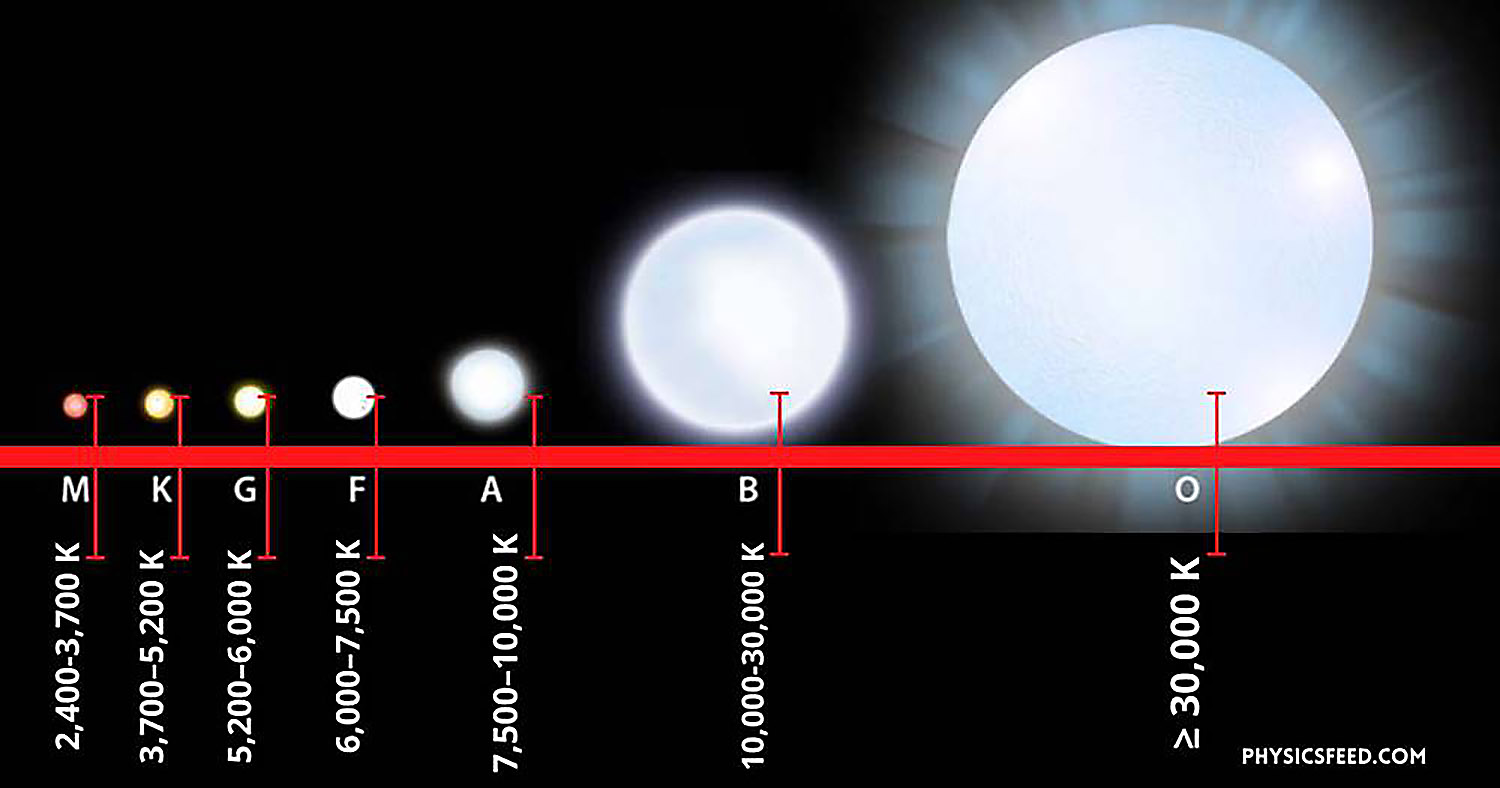
\includegraphics[height=0.65\textheight]{images/klase_zvezda.jpg}}
    \usebox0
    \captionsetup{width=\wd0}
    \caption{Главне спектралне класе са одговарајућим температурама, апроксимативним бојама и релативним величинама звезде}
  \end{figure}
\end{frame}

\end{document}
